\documentclass[notes=hide,hyperref={dvipdfmx,pdfpagelabels=false}]{beamer}
\title{Einführung in Sage - Einheit 9}
\subtitle{Strings, interaktive Grafiken, GeoGebra, Komplexe Beispiele}
\mode<article>
{
  \usepackage{fullpage}
  \usepackage{pgf}
  \usepackage[xetex]{hyperref}
  \setjobnamebeamerversion{beamer}
}

\mode<presentation>
{
  %\usetheme{Frankfurt}
 %\usetheme{My}
  \usetheme{Madrid}
  % or ...
%\usecolortheme{seagull}
  %\setbeamercovered{transparent}
  %\setbeamercovered{dynamic}
  % or whatever (possibly just delete it)
}
\usenavigationsymbolstemplate{}
\usefonttheme{structurebold}
\usepackage{multimedia}
%\usepackage{tikz}
\usepackage{fontspec,xunicode,xltxtra}

%\usepackage{polyglossia}
%\setdefaultlanguage[spelling=new, latesthyphen=true]{german}
%\setsansfont{DejaVu Sans}
%\setsansfont{Verdana}
%\setsansfont{Arial}
%\setromanfont{Linux Libertine O}
%\setsansfont{Linux Biolinum O}

\setbeamertemplate{footline}
{
\leavevmode
%\hbox{\begin{beamercolorbox}[wd=.5\paperwidth,ht=2.5ex,dp=1.125ex,
%leftskip=.3cm plus1fill,rightskip=.3cm]{author in head/foot}%
%    \usebeamerfont{author in head/foot}\insertshortauthor
%  \end{beamercolorbox}%
%  \begin{beamercolorbox}[wd=.5\paperwidth,ht=2.5ex,dp=1.125ex,leftskip=.3cm,
%rightskip=.3cm plus1fil]{title in head/foot}%
%    \usebeamerfont{title in head/foot}\insertshorttitle\hfill

\hfill\insertframenumber  \hspace{3pt}

%\inserttotalframenumber
%\hspace*{2ex}
%  \end{beamercolorbox}}%
  \vskip3pt%
}

\usepackage[ngerman]{babel}
\selectlanguage{ngerman}

%
% math/symbols
%
\usepackage{amssymb}
\usepackage{amsthm}
% \usepackage{latexsym}
\usepackage{amsmath}
%\usepackage{amsxtra} %Weitere Extrasymbole
%\usepackage{empheq} %Gleichungen hervorheben
%\usepackage{bm}
 %\bm{A} Boldface im Mathemodus

\usepackage{cellspace}
\setlength{\cellspacetoplimit}{2pt}
\setlength{\cellspacebottomlimit}{2pt}

%%%%%%%%%%%%%%%%%% Fuer Frames [fragile]-Option verwenden!
%Programm-Listing
%%%%%%%%%%%%%%%%%%
%Listingsumgebung fuer verbatim
%Grauhinterlegeter Text
%Automatischer Zeilenumbruch ist aktiviert
\usepackage{listings}
\definecolor{lgray}{gray}{0.80}
%\lstset{backgroundcolor=\color{lgray}, frame=single, basicstyle=\ttfamily, breaklines=true}
\lstnewenvironment{sage}{\lstset{backgroundcolor=\color{lgray},language=Python, emphstyle=\color{red}, frame=single, basicstyle=\ttfamily, breaklines=true,mathescape =true,escapechar=§}}{}


\usepackage{mydef}
%\usepackage{cmap} % you can search in the pdf for umlauts and ligatures
\usepackage{colonequals} %corrects the definition-symbols \colonequals (besides others)
\title{Einführung in Sage}
%
%\subtitle{Disputation} % (optional)

\author{Jochen Schulz}
% - Use the \inst{?} command only if the authors have different
%   affiliation.

\institute{Georg-August Universit\"at G\"ottingen \pgfimage[height=0.5cm]{../figures/unilogo3}}
% - Use the \inst command only if there are several affiliations.
% - Keep it simple, no one is interested in your street address.

\date{\today}

\subject{Sage}
% This is only inserted into the PDF information catalog. Can be left
% out. 

% If you have a file called "university-logo-filename.xxx", where xxx
% is a graphic format that can be processed by latex or pdflatex,
% resp., then you can add a logo as follows:

%\logo{\pgfimage[height=0.5cm]{figures/unilogo3}}


% Delete this, if you do not want the table of contents to pop up at
% the beginning of each subsection:

\AtBeginSection[]
{
  \begin{frame}<beamer>
    \frametitle{Aufbau}
    \tableofcontents[currentsection,currentsubsection]
  \end{frame}
}

\AtBeginSubsection[]
{
  \begin{frame}<beamer>
    \frametitle{Aufbau}
    \tableofcontents[currentsection,currentsubsection]
  \end{frame}
}



%%%%%%%%%%%%%%%%%%%
%Neue Definitionen
%%%%%%%%%%%%%%%%%%%

%Newcommands
\newcommand{\Fun}[1]{\mathcal{#1}}      %Mathcal fuer Funktoren
\newcommand{\field}[1]{\mathbb{#1}}     %Grundkoerper ?? in mathds

\newcommand{\A}{\field{A}}              %Affines A
\newcommand{\C}{\field{C}}              %Complexes C
\newcommand{\Fp}{\field{F}_{\!p}}       %Endlicher Koerper mit p Elementen
\newcommand{\Fq}{\field{F}_{\!q}}       %Endlicher Koerper mit q Elementen
\newcommand{\Ga}{\field{G}_{a}}         %Add Gruppenschema
\newcommand{\K}{\field{K}}              %Generischer Koerper 
\newcommand{\N}{\field{N}}              %Nat Zahlen
\newcommand{\Pj}{\field{P}}             %Projektives P
\newcommand{\R}{\field{R}} 		%Reelle Zahlen
\newcommand{\Q}{\field{Q}}              %Rationale Zahlen  
\newcommand{\Qt}{\field{H}}             %Quaternionen 
\newcommand{\V}{\field{V}}              %Vektorbuendel V
\newcommand{\Z}{\field{Z}}              %Ganze Zahlen

\newcommand{\fdg}{\;|\;}                 %fuer die gilt

%Operatoren
\DeclareMathOperator{\Abb}{Abb}
%\usepackage{sagetex}

\begin{document}
\lstset{basicstyle={\lstbasicfont\footnotesize}}


\maketitle

\begin{frame}{Aufbau}
\tableofcontents
\end{frame}

\begin{frame}{Klausur}
 \begin{itemize}
\item Zeit: 10.03.2011 von 10:30 - 12:00
\item  Ort: HS1 (A bis J) und AudiMax (K bis Z)
\item  Hilfsmittel: Schreibgerät(e) und Unterlagen in Papierform
\item  Studenten-Ausweis mitbringen
\item Schreibweisen der art $x^2$ oder $xy$ sind ok, solange klar ist was gemeint ist.
%\item  Ab 10:30 keine vorzeitige Abgabe möglich
\end{itemize}

\end{frame}

%===================================================
\section{Umgang mit Strings}
%==================================================

\begin{frame}[fragile]{Strings}
\begin{itemize}
\item Zeichenketten (engl. {\color{red} strings}) sind eine geordnete
Aneinanderreihung von Zeichen. Zeichen sind z.B. Buchstaben, Ziffern,
Sonderzeichen,...
\item Mit ihnen kann man in Sage Texte gestalten. Sie sind wichtig
für die Ausgabe der Ergebnisse.
\item Datentyp \isage{str}.
\item eingeschlossen in Hochkommas oder Anführungszeichen.
\end{itemize}
\end{frame} 


\begin{frame}[fragile]{Beispiele für Strings}
\begin{sagein}
text1 = 'Dies ist ein String.'; text1
\end{sagein}
\begin{sage}
'Dies ist ein String.'
\end{sage}
\begin{sagein}
text2 = "Dies ist noch ein String."; text2
\end{sagein}
\begin{sage}
'Dies ist noch ein String.'
\end{sage}
\begin{sagein}
type(text1)
\end{sagein}
\begin{sage}
<type 'str'>
\end{sage}
\end{frame}

\begin{frame}[fragile]{Zugriff}
\begin{itemize}
\item Indexoperator {\color{blue}$[\ ]$}:
\begin{sagein}
text1[0], text1[3], text1[2:4], text1[0:4:2]
\end{sagein}
\begin{sage}
('D', 's', 'es', 'De')
\end{sage}
\item Ersetzungen innerhalb des Strings:
\begin{sagein}
text1.replace('Dies','Das')
\end{sagein}
\begin{sage}
'Das ist ein String.'
\end{sage}
\end{itemize}
\end{frame}

\begin{frame}[fragile]{Operationen für Strings I}
\begin{itemize}
\item Zusammenhängen von Strings
\begin{sagein}
A='Letzte '; B='Vorlesung'; A+B
\end{sagein}
\begin{sage}
'Letzte Vorlesung'
\end{sage}
\item \isage{len()} gibt die Anzahl der Zeichen in einer Zeichenkette
an.
\begin{sagein}
a=len(A+B); a
\end{sagein}
\begin{sage}
  16
\end{sage}
 
\end{itemize}
\end{frame}

\begin{frame}[fragile]{Operationen für Strings II}
\begin{itemize}
\item Zugriffe beginnend vom Ende
\begin{sagein}
(A+B)[-1]
\end{sagein}
\begin{sage}
  'g'
\end{sage}
\item {\color{blue} \isage{str()}} wandelt Objekte in einen String um.
\begin{sagein}
str(x^2+2), str([1,2,3])
\end{sagein}
\begin{sage}
('x^2 + 2', '[1, 2, 3]')
\end{sage}
\end{itemize}
\end{frame}

\begin{frame}[fragile]{Operationen für Strings III}
\begin{itemize}
 \item \isage{find()}: Strings durchsuchen
\begin{sagein}
'Hallo'.find('lo')
\end{sagein}
\begin{sage}
3
\end{sage}
\item 
\begin{sagein}
'Hallo'.find('gnu')
\end{sagein}
\begin{sage}
-1
\end{sage}
\end{itemize}
\end{frame}

\begin{frame}[fragile]{Operationen für Strings IV} 
\begin{itemize}
\item \isage{split()}: Aufspalten von Texten
\begin{sagein}
text = 'Dies ist ein Satz, und ein Nebensatz'
text.split() 
\end{sagein}
\begin{sage}
 ['Dies', 'ist', 'ein', 'Satz,', 'und', 'ein', 'Nebensatz']
\end{sage}
\begin{sagein}
text.split('i')
\end{sagein}
\begin{sage}
['D', 'es ', 'st e', 'n Satz, und e', 'n Nebensatz']
\end{sage}

\end{itemize}
\end{frame}


\begin{frame}[fragile]{Vertiefung print und Formate} 
 \begin{sagein}
  print 'Text %<format> und %<format> ... ' % (x,y,...)
 \end{sagein}
\isage{<format>}:
\begin{sagein}
%[<flag>][<minwidth>][.<precision>]converter 
\end{sagein}
\begin{itemize}
\item \isage{flag}: 0 für das Auffüllen mit Nullen
\item \isage{minwidth}: Minimale Breite der Darstellung
\item \isage{precision}: Genauigkeit (Nachkommastellen)
\item \isage{converter}:
\begin{tabular}{cp{10cm}}
\isage{'i'} & ganze Zahl mit Vorzeichen\\
\isage{'e'} & Gleitkommazahl mit exponentialformat (kleingeschrieben).\\
\isage{'f'} &Gleitkommazahl im Dezimalformat.\\
\isage{'g'} &Gleitkommazahl. Benutzt kleingeschriebene Exponentialform wenn der Exponent kleiner als -4 oder der Genauigkeit ist, ansonsten Dezimalformat.
\end{tabular}

\end{itemize}



\end{frame}

\begin{frame}[fragile]{print - Beispiele}
\begin{sagein}
print '%5s | %7s' % ('Index','Wert')
for k in srange(1,25,9.55): 
    print '%5i | %07.3f' % (k,k^2) 
\end{sagein}
\begin{sage}
Index |    Wert
    1 | 001.000
   10 | 111.303
   20 | 404.010
\end{sage}
 
\end{frame}



% \begin{frame}[fragile]{Anwendungen}
% \item Schreiben Sie eine Funktion, die eine Zeichenkette rückwärts
% berechnet. 
% \begin{sagein}
% revers:= A->_concat(A[length(A)-i+1]
%    $\text{dollar}$ i=1..length(A))
% \end{sagein}
% \begin{sagein}
% revers("Hallo")
% \end{sagein}
% \begin{sage}
%   "ollaH"
% \end{sage}
% \end{itemize}
% \end{frame}

\section{Interaktive (grafische) Elemente}

\begin{frame}[fragile]{interact}
\begin{sagein}
@interact
def _(b = range_slider(-20, 20, 1, default=(-19,3), label='Range')):
    plot(sin(x)/x, b[0], b[1]).show(xmin=b[0],xmax=b[1]) 
\end{sagein}
\begin{center}
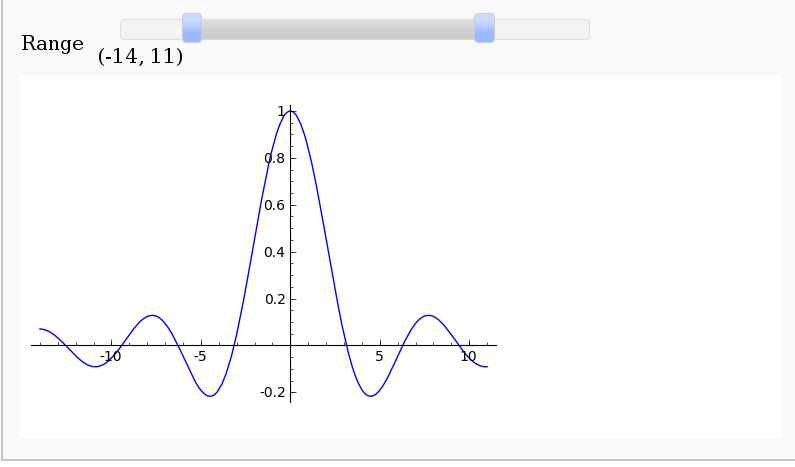
\includegraphics[width=0.8\textwidth]{figures/interact_basis.png}
\end{center}

\end{frame}


\begin{frame}[fragile]{interact}
\begin{itemize}
\item Regler mit Werten von vmin bis vmax
\begin{sagein}
u=slider(vmin, vmax=, step_size=1, default=, label=) 
\end{sagein}
\item Regler eines Intervalles
\begin{sagein}
u=range_slider(vmin, vmax=, step_size=1, default=, label=)
\end{sagein}
\item Eine Ankreuzfeld
\begin{sagein}
u=checkbox(default=True, label=)
\end{sagein}
\item Ein Aufklappmenü oder Knöpfe (Knöpfe wenn nrows, ncols, oder buttons gesetzt ist, sonst Aufklappmenü)
\begin{sagein}
u=selector(values, label=, nrows=, ncols=, buttons=False)
\end{sagein}
\item Ein Textblock
\begin{sagein}
u=text_control(value='')
\end{sagein}

\end{itemize}


\end{frame}



\begin{frame}[fragile]{interact - Taylor}
\begin{center}
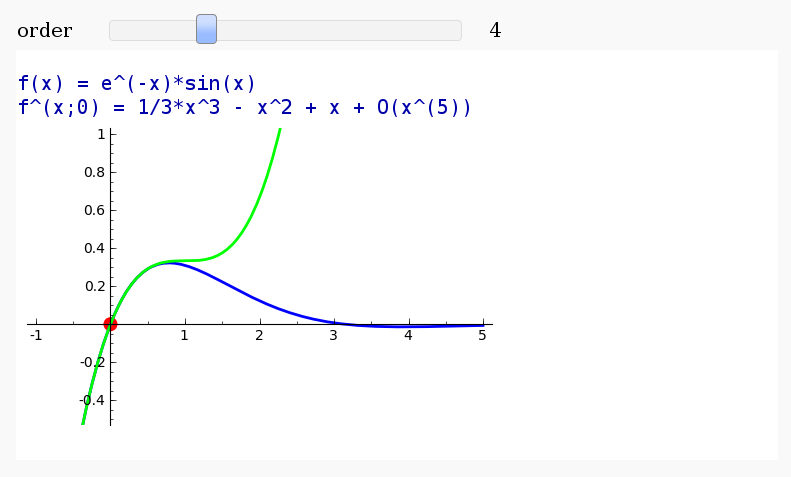
\includegraphics[width=\textwidth]{figures/interact1.png}
\end{center}
\end{frame}


\begin{frame}[fragile]{interact - Taylor}
\begin{sagein}
var('x')
x0  = 0
f   = sin(x)*e^(-x)
p   = plot(f,-1,5, thickness=2)
dot = point((x0,f(x=x0)),pointsize=80,rgbcolor=(1,0,0))
@interact
def tayl(order=slider(1,12,1,label='order')):
    ft = f.taylor(x,x0,order)
    pt = plot(ft,-1, 5, color='green', thickness=2)
    print ('f(x) = %s'% f)
    print ('f^(x;%s) = %s + O(x^(%s))'%(x0,ft,order+1))
    show(dot + p + pt, ymin = -.5, ymax = 1)
\end{sagein}
\end{frame}

\begin{frame}[fragile]{interact - Grafiken von einer Abstandsfunktion}
\begin{center}
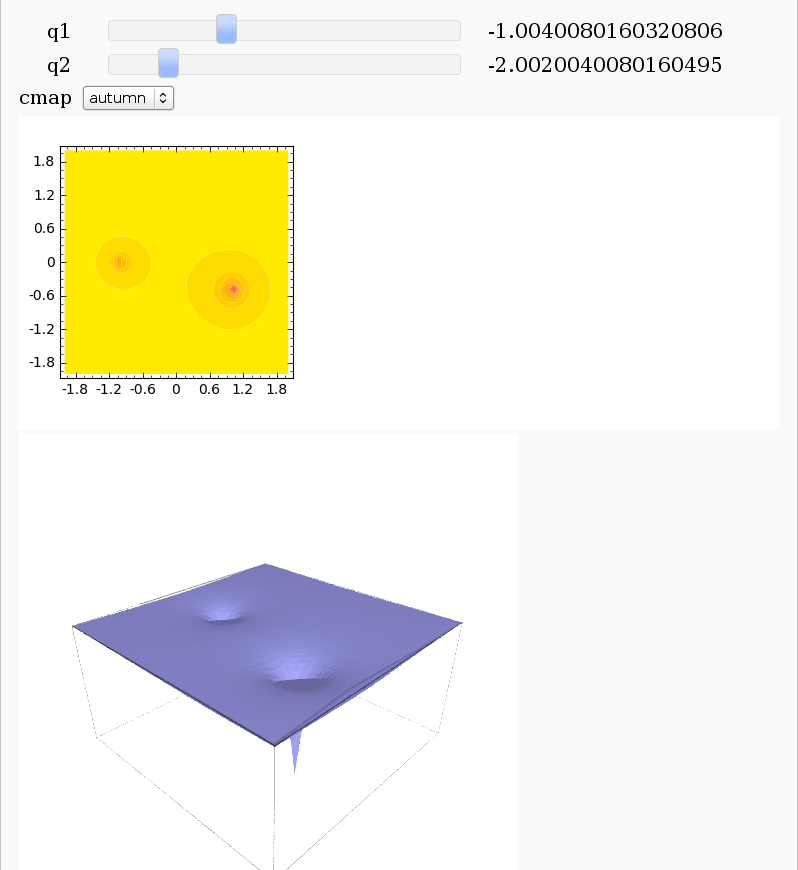
\includegraphics[width=7.5cm]{figures/interact2.png}
\end{center}
\end{frame}


\begin{frame}[fragile]{interact - Grafiken von einer Abstandsfunktion}
\begin{sagein}
@interact
def _(q1=slider(-3,3,default=-1), q2=slider(-3,3,default=-2), cmap=selector(['autumn', 'bone', 'cool', 'copper', 'gray', 'hot', 'hsv','jet', 'pink', 'prism', 'spring', 'summer','winter'])):
     x,y = var('x,y')
     f = q1/sqrt((x+1)^2 + y^2) + q2/sqrt((x-1)^2+(y+0.5)^2)
     C = contour_plot(f, (x,-2,2), (y,-2,2), plot_points=30, contours=15, cmap=cmap)
     show(C, figsize=3, aspect_ratio=1)
     show(plot3d(f, (x,-2,2), (y,-2,2)), figsize=5, viewer='tachyon')
\end{sagein}

\end{frame}

\section{GeoGebra}

\begin{frame}[fragile]{GeoGebra einbetten}
\begin{itemize}
 \item In GeoGebra: Erstellen eines Objektes
\item In GeoGebra: File> Export> Dynamic worksheet.
\item In Sage notebook: Data> Die .jar (von GeoGebra) und die .ggb hochladen.
\item Aus dem Exportierten .html den Teil mit <applet> kopieren und im worksheet in Sage unter Edit kopieren( Edit> Paste ).
\item Im Editier-tab die codebase zu "./data/" ändern
\item Fertig!
\end{itemize}
 
\end{frame}

\begin{frame}[fragile]{GeoGebra einbetten}
\begin{center}
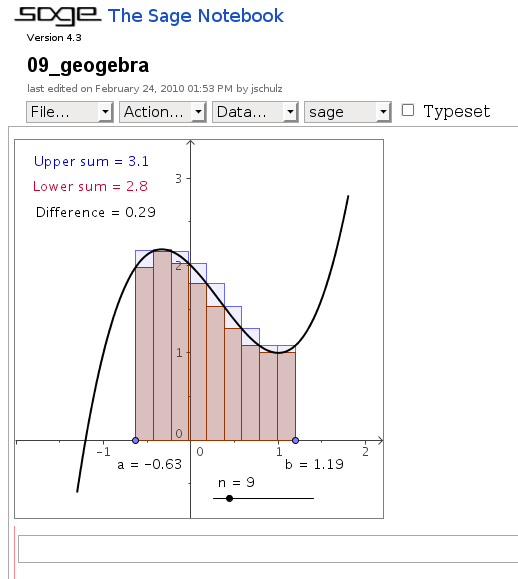
\includegraphics[width=0.6\textwidth]{figures/geogebra.png}
\end{center}
\end{frame}


%%%%%%%%%%%%%%%%%%%%%%%%%%%%%%%%%%%%%%%%%%
\section{Vertiefung Programmierung}
%%%%%%%%%%%%%%%%%%%%%%%%%%%%%%%%%%%%%%%%%%

\begin{frame}[fragile]{Größter gemeinsamer Teiler (ggT)}
Berechnung des ggT von natürlichen Zahlen $a$ und $b$ mit Hilfe des
euklidischen Algorithmus.
\bigskip

\textbf{Idee:} Es gilt:
\begin{enumerate}
 \item $ggT(a,b)=ggT(a,b-a)$ für $a<b$.
\item $ggT(a,b)=ggT(b,a)$.
\item $ggT(a,a)=a$.
\end{enumerate}

\textbf{Algorithmus:}

Wiederhole,  bis $a=b$
 \begin{itemize}
\item Ist $a>b$, so $a=a-b$.
\item Ist $a<b$, so $b=b-a$ 
\end{itemize}
\end{frame}

\begin{frame}[fragile]{ggT - Implementierung}
\begin{sagein}
def ggT(a,b):  
    """Bestimme den ggT von a und b"""
    while a<>b:
        if a>b:
            a = a-b
        else: 
            b = b-a
    return a
ggT(6,9)
\end{sagein}
\begin{sage}
3  
\end{sage}

\end{frame}




% %-----------------------------
% \subsection{Schleifen}
% %----------------------------
% 
% \begin{frame}[fragile]{Repeat}
% Neben \isage{for} ist durch  \isage{repeat} eine weitere Schleifenvariante gegeben:
% \begin{sage}
% x:=1.1:
% repeat
%   i:=x; x:=i^2; print(i,x)
% until x>100 end_repeat:
% \end{sage}
% Die Befehle zwischen \isage{repeat} und \isage{until} werden so lange
% wiederholt, bis die Bedingung (hier $x>100$) wahr wird.
% \end{frame}
% 
% \begin{frame}[fragile]{while}
% So ähnlich wie die \isage{repeat}-Schleife funktioniert die
% \isage{while}-Schleife. 
% \begin{sage}
% x:=2:
% while x<=100 do
%  i:=x; x:=i^2; print(i,x)
% end_while:
% \end{sage}
% Die Befehle zwischen \isage{while} und \isage{end_while} werden so lange
% wiederholt, wie die Bedingung (hier $x<=100$) wahr ist.
% \end{frame}
% 
% \begin{frame}[fragile]{Verzweigung}
% \begin{itemize}
% \item Ein wichtiges Werkzeug jeder Programmiersprache sind
% Verzweigungen. 
% \item Je
% nach Wert oder Bedeutung von Variablen werden unterschiedliche Befehle
% ausgeführt. 
% \item In MuPAD gibt es das \isage{if}-Konstrukt und das \isage{case}-Konstrukt. 
% \end{itemize}
% \end{frame}

% \begin{frame}[fragile]{Beispiel}
% \begin{sage}
% for i from 2 to 100 do
%  if isprime(i)
%    then print(i,"ist Primzahl")
%    else print(i,"ist keine Primzahl")
%  end_if
% end_for:
% \end{sage}
% \end{frame}
% 

\begin{frame}[fragile]{Berechnung von Primzahlzwillingen}
\begin{sagein}
T = []; anz = 0
for i in [2..100]:
    if (is_prime(i) and is_prime(i+2)):
        anz += 1
        T.append([i,i+2])
print('Anzahl = %s' % anz);T
\end{sagein}
\begin{sage}
Anzahl = 8
[[3, 5], [5, 7], [11, 13], [17, 19], [29, 31], [41, 43], [59, 61], [71,
73]]
\end{sage}

\end{frame}

% \begin{frame}[fragile]{Case}
% Hat man eine Verzweigung mit mehreren Alternativen, so kann man
% entweder geschachtelte \isage{if} Konstrukte verwenden, oder das
% Konstrukt \isage{case} verwenden. 
% 
% \begin{sage}
% case var
%  of wert1 do ...
%  of wert2 do ...
%     ...
%  otherwise
%     ...
% end_case
% \end{sage}
% \isage{Case} funktioniert wie die \isage{switch} Anweisung in C.
% \end{frame}

\begin{frame}[fragile]{Betrag}
\begin{sagein}
def betrag(a):
    if a in ZZ or a in QQ or a in RR:
        if a>0:
            y = a
        else:
            y = -a
    elif a in CC:
        y = sqrt(real(a)^2+imag(a)^2)
    else:
        return 'Falscher Eingabetyp'
    return y
betrag([1,2]), betrag(2+I*2)
\end{sagein}
\begin{sage}
('Falscher Eingabetyp', 2*sqrt(2))
\end{sage}
\end{frame}


% \begin{frame}[fragile]{Erklärungen}
% \begin{itemize}
% \item Durch \isage{args()} erhält man die Folge der Argumente. 
% \item \isage{args(0)} ist die Anzahl der Argumente.
% \item Durch \isage{args(i)} erhält man das $i$-te Element.
% \item Mit diesen Befehlen kann man Prozeduren mit einer beliebigen
% Anzahl von Argumenten programmieren.
% \item \isage{procname} ist der Name der Prozedur.
% \end{itemize}
% \end{frame}

% \begin{frame}[fragile]{Testen des Typs}
% Durch den Aufruf
% \begin{sage}
% testtype(Objekt, Typenbezeichner)
% \end{sage}
% wird getestet, ob ein \isage{Objekt} dem Typenbezeichner
% entspricht. Rückgabewert ist \isage{TRUE} oder \isage{FALSE}.
% \begin{itemize}
% \item Prinzipiell kann man auch \isage{domtype} zum Überprüfen des Typs
% benutzen. 
% \item Die Typenbezeichner sind aber differenzierter.
% \item Übersicht der verfügbaren Typenbezeichner erhält man durch
% {\color{blue} \isage{? Type}}. 
% \end{itemize}
% \end{frame}

% \begin{frame}[fragile]{Beispiele}
% \begin{sagein}
% testtype(sqrt(3),Type::Real)
% \end{sagein}
% \begin{sage}
%   FALSE
% \end{sage}
% \begin{sagein}
% testtype(float(sqrt(3)),Type::Real)
% \end{sagein}
% \begin{sage}
%   TRUE
% \end{sage}
% \begin{sagein}
% testtype(3,Type::Real)
% \end{sagein}
% \begin{sage}
%   TRUE 
% \end{sage}
% \begin{sagein}
% select([i $\text{dollar}$ i=100..120],testtype,Type::Prime)
% \end{sagein}
% \begin{sage}
%   [101, 103, 107, 109, 113]
% \end{sage} 
% \end{frame}


\begin{frame}[fragile]{Mandelbrot-Menge}
Die Mandelbrot-Menge ist die Menge von Punkten $c \in \mathbb{C}$
bei denen die Folge $(z_n)_n$, die durch
\[ z_0:=c, \qquad  z_{n+1} = z_n^2 +c, \quad n \in \mathbb{N}\]
definiert ist, beschränkt ist.
\end{frame}

\begin{frame}[fragile]{Programm - Mandelbrot}
\begin{sagein}
def mandel(x,y):
    c = (x + I*y).n()
    z = c
    it = 0
    max_it = 150
    while abs(z)<2 and it<max_it:
        z = z^2 + c
        it += 1
    return float(it/max_it)
\end{sagein}
Die Funktion \isage{mandel} gibt zu $x+iy$ die relative Anzahl der
Iterationsschritte zurück.
\end{frame}

\begin{frame}[fragile]{Plot - Mandelbrot}
\begin{sagein}
density_plot(mandel, (-2.1,1.2), (-1.1,1.1), plot_points=100)
\end{sagein}
\begin{center}
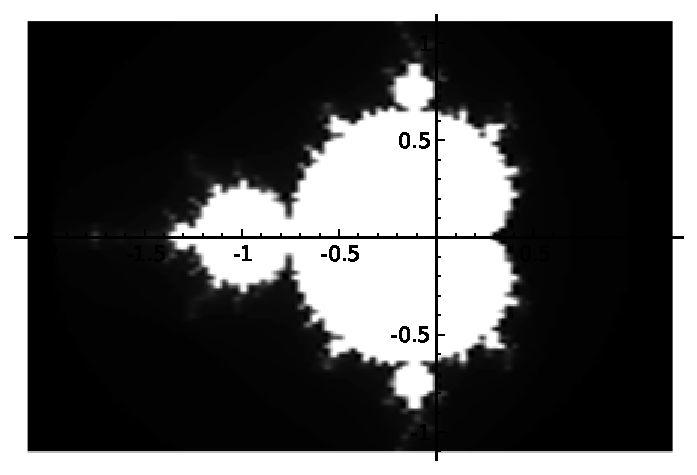
\includegraphics[width=0.8\textwidth]{figures/mandel.pdf} 
\end{center}

\end{frame}


\begin{frame}[fragile]{Letztes Beispiel I}
\begin{sagein}
def Gadisch(x,basis):
    """Berechnung der Darstellung einer natuerlichen Zahl 
x zur Basis b. Rueckgabe des Ergebnis als Liste!"""
    #Abfangen der Eingabe
    if not x in ZZ or x < 0 or basis==1: 
        return 'Eingabe nicht korrekt!'
    T = []  # leere Liste 
    while x>0:
        T.append(x%basis) # Rest der Division
        print '%i : %i = %i Rest %i' % (x,basis,floor(x/basis),x%basis)
        x = floor(x/basis) # Teiler setzen
    # Rueckgabe der Liste
    return T
\end{sagein}
\end{frame}

\begin{frame}[fragile]{Letztes Beispiel II}
\begin{sagein}
Gadisch(6,2)
\end{sagein}
\begin{sage}
6 : 2 = 3 Rest 0
3 : 2 = 1 Rest 1
1 : 2 = 0 Rest 1
[0, 1, 1]
\end{sage}

\begin{sagein}
Gadisch(3.4,2)
\end{sagein}
\begin{sage}
'Eingabe nicht korrekt!'
\end{sage}


\end{frame}

\begin{frame}{Allerletztes Beispiel: Kochsche Kurven I}
\begin{itemize}
\item Seien $y_1,y_2$ zwei Punkte im $\mathbb{R}^2$. 
\item Betrachte die Strecke mit Endpunkten $y_1$ und $y_2$.  
\item Ersetze  diese Strecke durch 4 Strecken 
$\overline{y_1 z_1}$, $\overline{z_1 z_2}$, $\overline{z_2 z_3}$,
$\overline{z_3 y_2}$ mit Endpunkten 
\begin{eqnarray*}
 z_1 &=&\frac23 y_1 + \frac13 y_2\\[0.5cm]
 z_2 &=& \frac{\sqrt{3}}{6} \left( \begin{array}{cc}
 0 & 1 \\ -1 & 0 \\
 \end{array} \right)
 (y_1 - y_2) + \frac12 (y_1 + y_2)\\[0.5cm]
 z_3 &=&\frac13 y_1 + \frac23 y_2
\end{eqnarray*}
\item Dieses Prozedere wird nun für jede einzelne Teilstrecke wiederholt.
\end{itemize}
\end{frame}

\begin{frame}[fragile]{Allerletztes Beispiel II}
\begin{sagein}
def koch(y1,y2,lev):
    Listelinien = []
    if (lev == 0):
        Listelinien.append(line([(y1[0],y1[1]),(y2[0],y2[1])]))
    else:
        # Definieren der neuen Punkte 
        z1 = 2/3 * y1 + 1/3 * y2
        z3 = 1/3 * y1 + 2/3 * y2
        z2 = sqrt(3)/6*matrix([[0, 1],[ -1, 0]])*(y1-y2) + 1/2 * (y1 + y2)
        # Definieren der 4 Strecken
        Listelinien.append(koch(y1, z1, lev-1))
        Listelinien.append(koch(z1, z2, lev-1))
        Listelinien.append(koch(z2, z3, lev-1))
        Listelinien.append(koch(z3, y2, lev-1))
    return add(Listelinien)
\end{sagein}
\end{frame}

\begin{frame}[fragile]{Allerletztes Beispiel III}
\begin{sagein}
# Einfacher Fall einer Linie 
koch(vector([0,0]),vector([1,0]),4)
\end{sagein}
\begin{center}
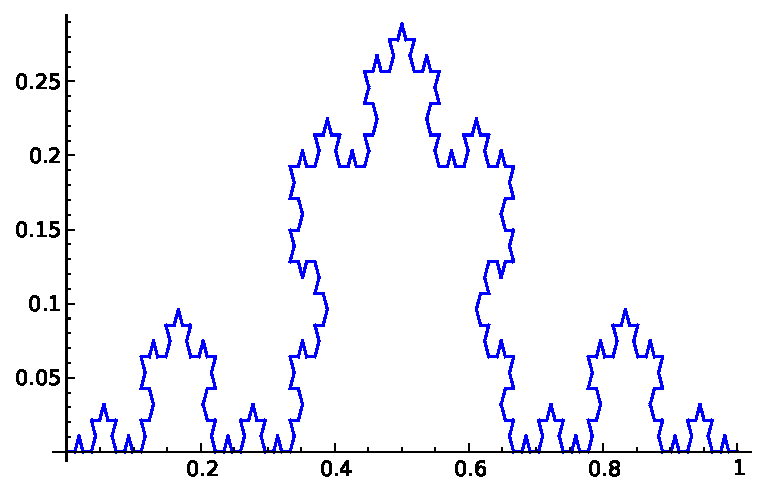
\includegraphics[width=0.7\textwidth]{figures/koch.pdf} 
\end{center}
\end{frame}
\end{document}
